\documentclass[letterpaper]{article}

\usepackage[english]{babel}
\usepackage[utf8]{inputenc}
\usepackage{amsmath}
\usepackage{graphicx}
\usepackage{subfig}
\usepackage{epsfig}
\usepackage[nottoc]{tocbibind}
\usepackage[colorinlistoftodos]{todonotes}
\usepackage[hidelinks]{hyperref}
\usepackage[margin=1in]{geometry}
% \setlength{\parindent}{0em}
\renewcommand{\floatpagefraction}{1}%

\title{Predicting the Direction of Exchange-Traded Fund (ETF) Movement}

\author{Kai Liu \\ The University of Texas at Austin}

\date{April 2017}

\newcommand{\gfigure}[4]
{
	\begin{figure}
      \centering
          \includegraphics[#3]{#4}
          \caption{#1}
          \label{Figure:#2}
    \end{figure}
}

\newcommand{\figref}[1]{Figure~\ref{Figure:#1}}

\begin{document}
\maketitle

\section{Summary}
In this project, I used machine learning techniques to predict the direction of
the following ETFs: XLE, XLU, XLK, XLB, XLP, XLY, XLI, XLV and SPY. In the
modeling process, two different types of input predictors are used in
predicting the directions. One type of predictors are OHLC prices, volume size
and weekday information, which is called pure data-driven method in the report.
The other types of predictors are weekday information and some technical
indicators chosen from literature, referred as indicator-driven method. In
addition, four different models are implemented: logistic regression, Lasso
regression, Ridge regression, and artificial neural network. Besides, though I
attempted to predict the direction, I also converted the binary dependent
variable into other two types to compare which type of dependent variable can
achieve the best performance. In conclusion, the accuracy of the best model
for each ETF sector ranges from 55\% to 60\%. And the trading strategy based on
my prediction earns less than the all long-only strategy, but it has a lower
risk to achieve the earning.

\section{Method}
\subsection{Data}
In the project, I attempted to predict the direction of the following ETFs:
XLE, XLU, XLK, XLB, XLP, XLY, XLI, XLV, and SPY. The daily OHLC (Open, High,
Low, Close) prices and volumes for these ETFs are obtained from Yahoo Finance.
The total number of samples is 4,277 trading days, from January 1st 2000 to
December 31st 2016. The total 4,277 data points of the daily OHLC prices and
volumes of the first two ETF sectors are plotted in Figure \ref{plotRawData}. I
divide each dataset into two parts, 94.1\% of the data (January 1st 2000 to
December 31st 2015) is used from in-sample training and 5.9\% (January 1st 2016
to December 31st 2016) are considered as out-of-sample data. The in-sample data
is used to train the models, while out-of-sample is reserved to evaluate
performance of models.

\begin{figure}
  % \centering
    \subfloat[XLE]{
        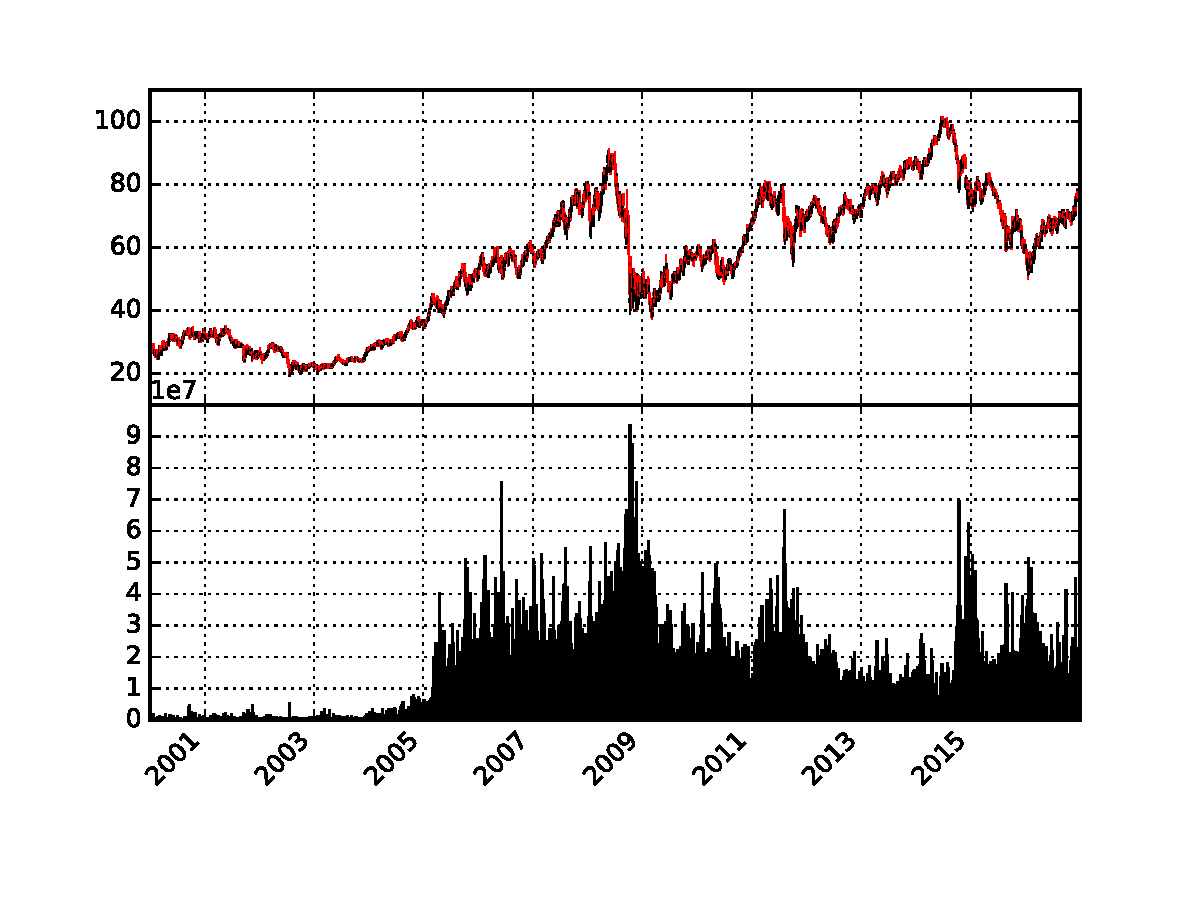
\includegraphics[width=3in]{Images/XLE_raw.pdf}
    }
    \subfloat[XLU]{
        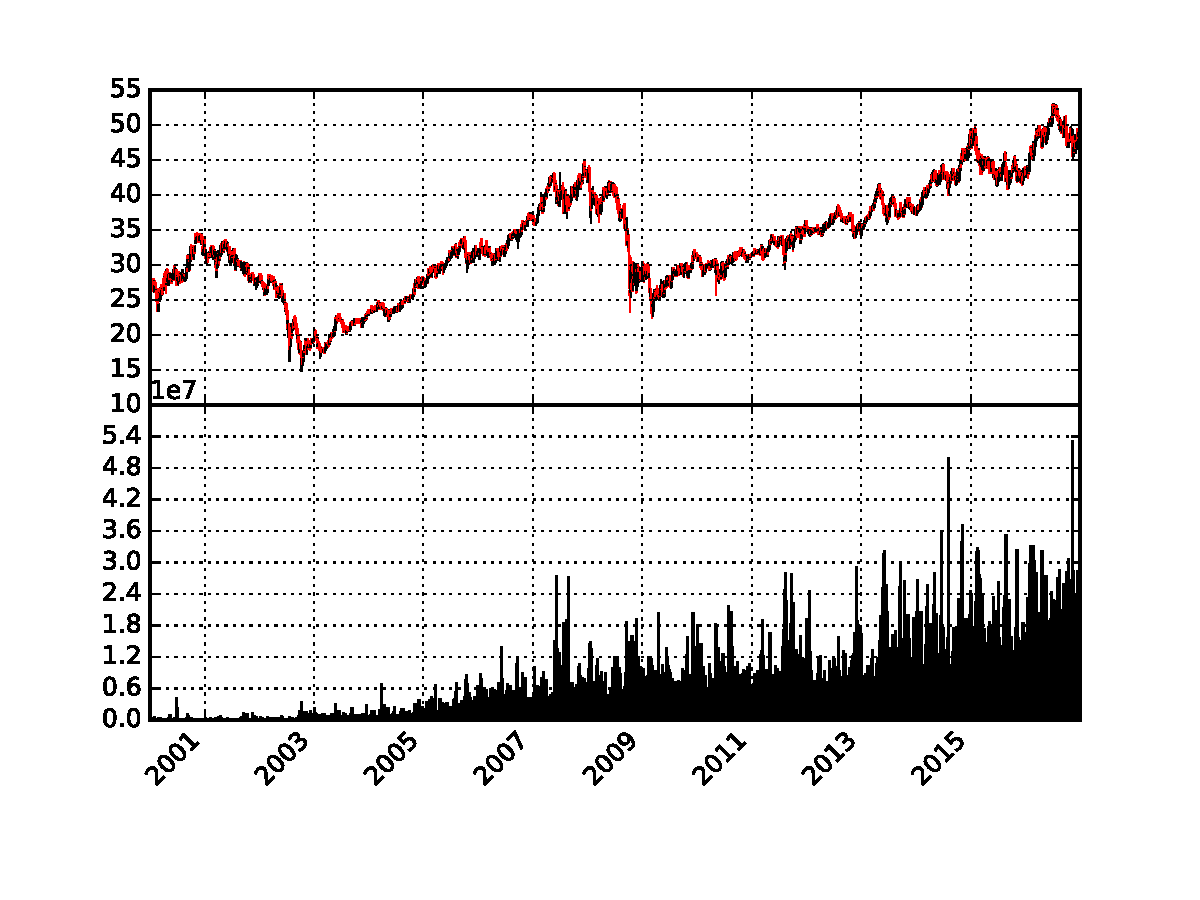
\includegraphics[width=3in]{Images/XLU_raw.pdf}
    } \\
    % \subfloat[XLK]{
        % 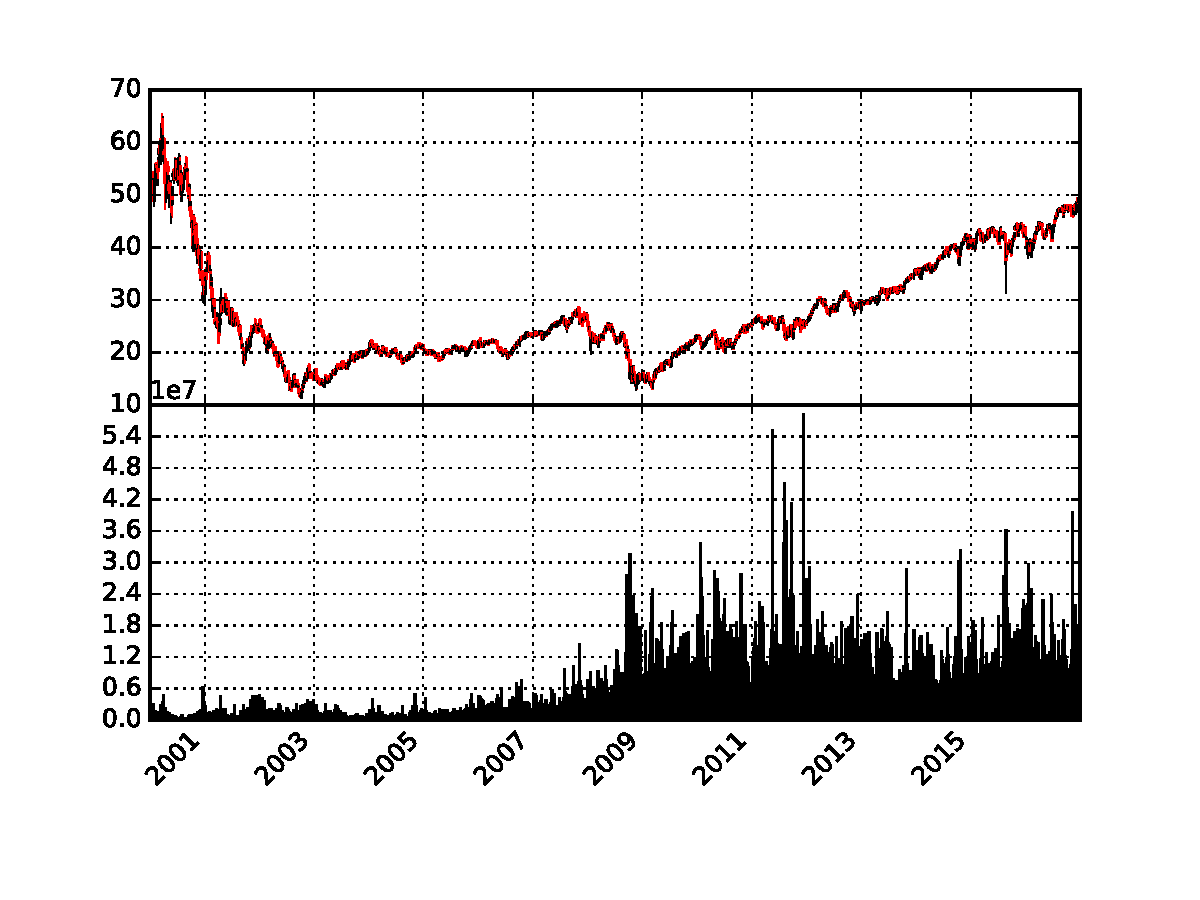
\includegraphics[width=3in]{Images/XLK_raw.pdf}
    % }
    % \subfloat[XLB]{
        % 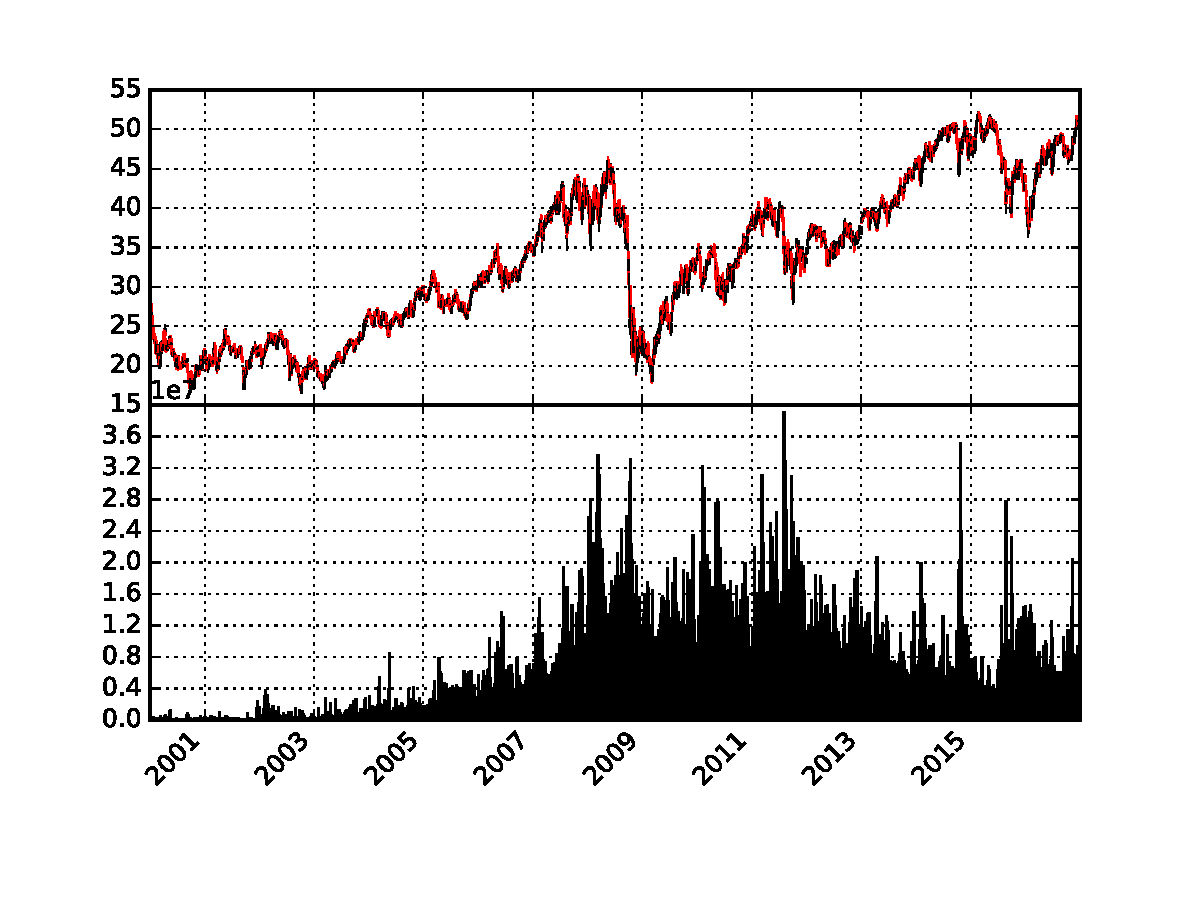
\includegraphics[width=3in]{Images/XLB_raw.pdf}
    % } \\
    % \subfloat[XLP]{
        % 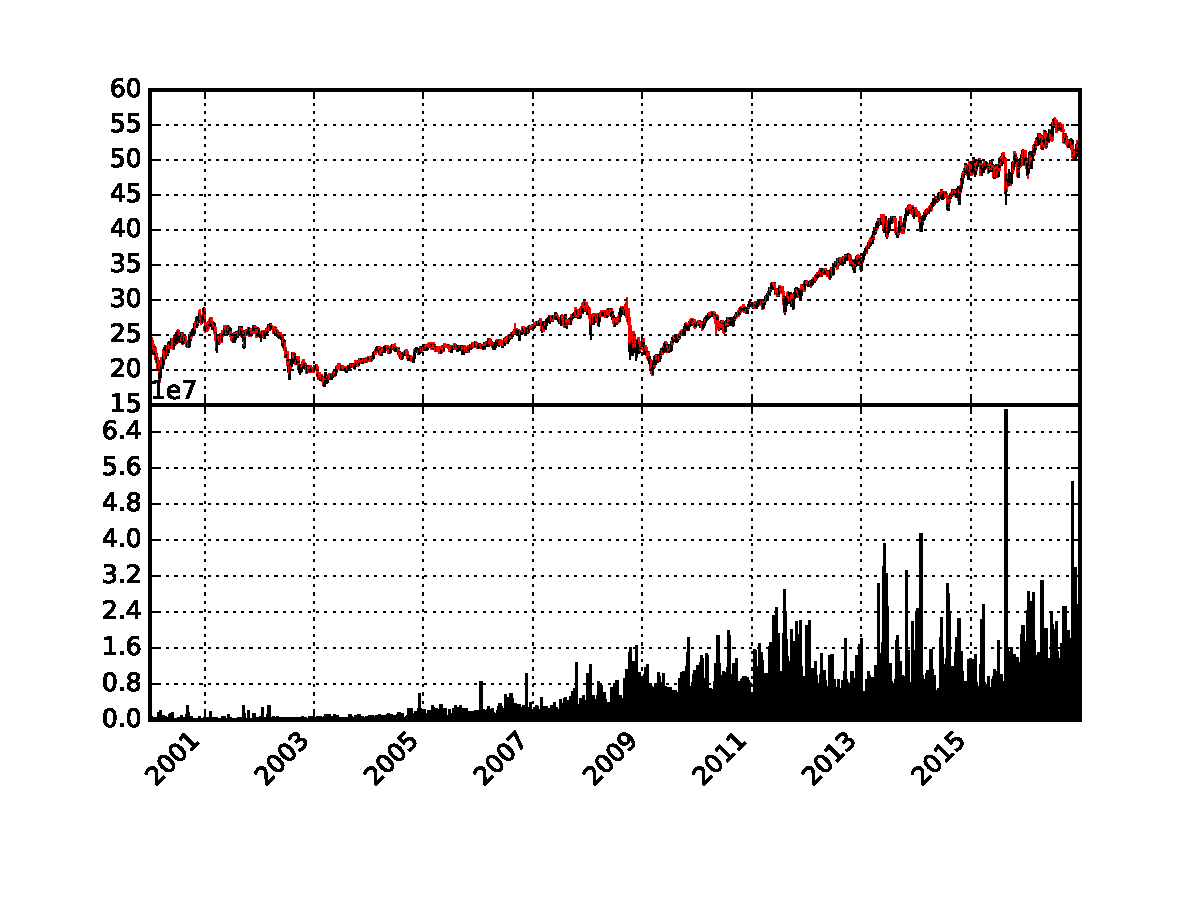
\includegraphics[width=3in]{Images/XLP_raw.pdf}
    % }
    % \subfloat[XLY]{
        % 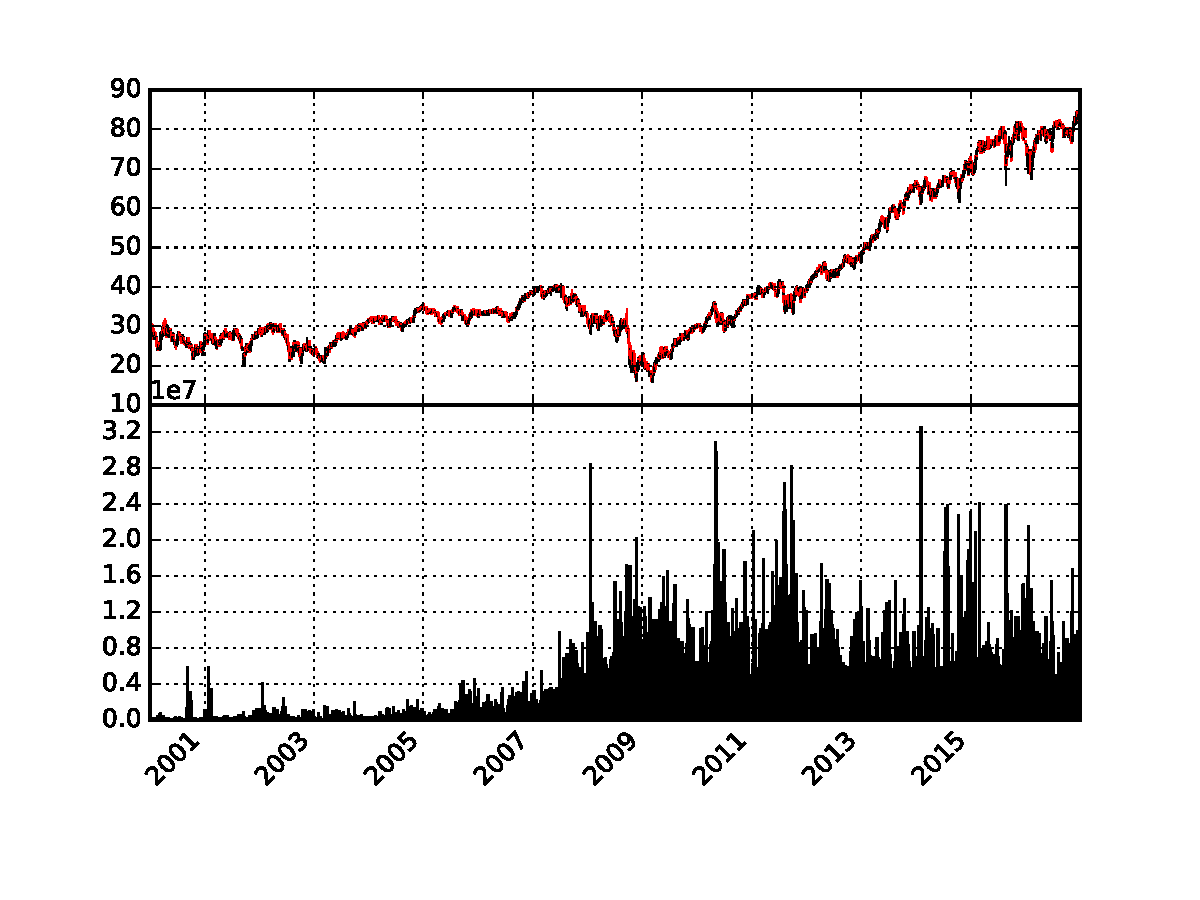
\includegraphics[width=3in]{Images/XLY_raw.pdf}
    % } \\
  % \caption{Raw data visualization}
  % \label{plotRawData}
% \end{figure}
% \begin{figure}
  % \ContinuedFloat
  % \centering
    % \subfloat[XLI]{
        % 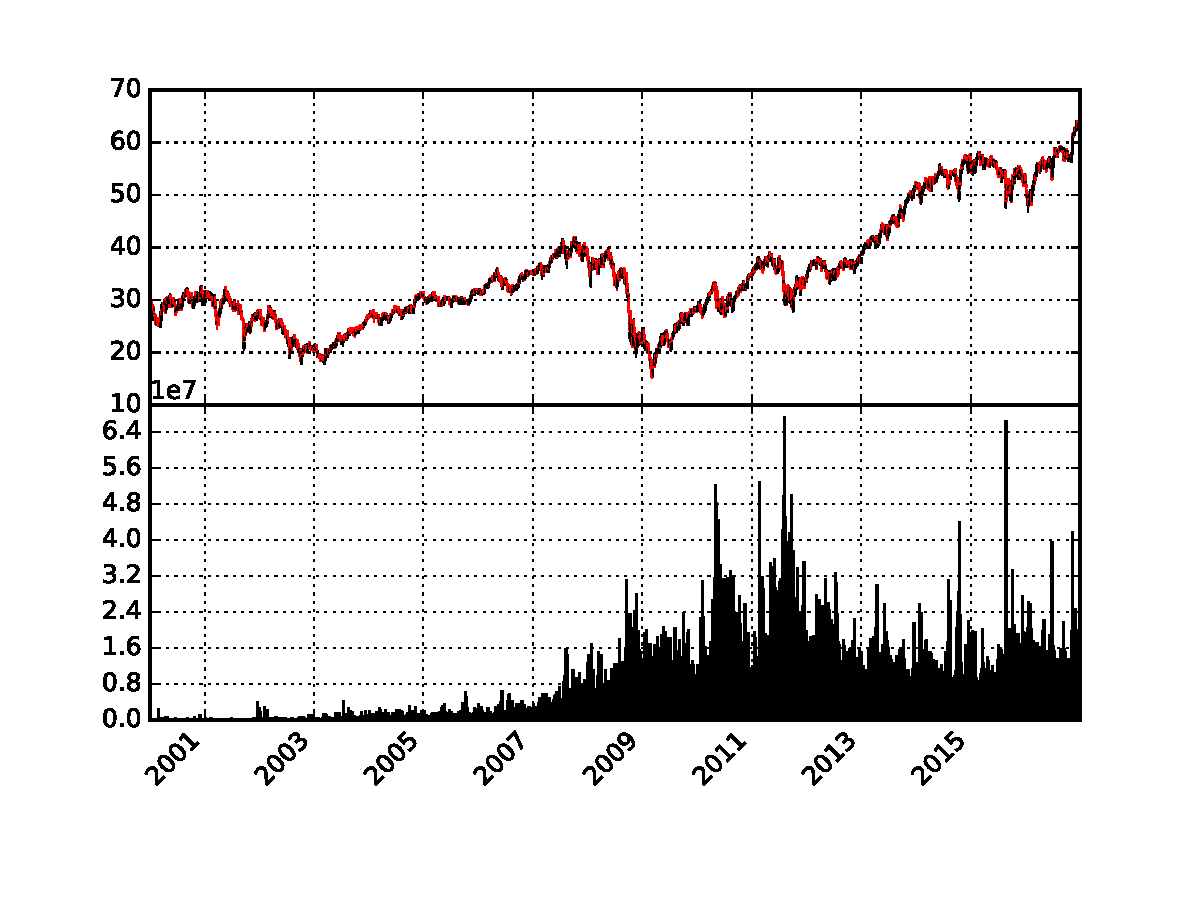
\includegraphics[width=3in]{Images/XLI_raw.pdf}
    % }
    % \subfloat[XLV]{
        % 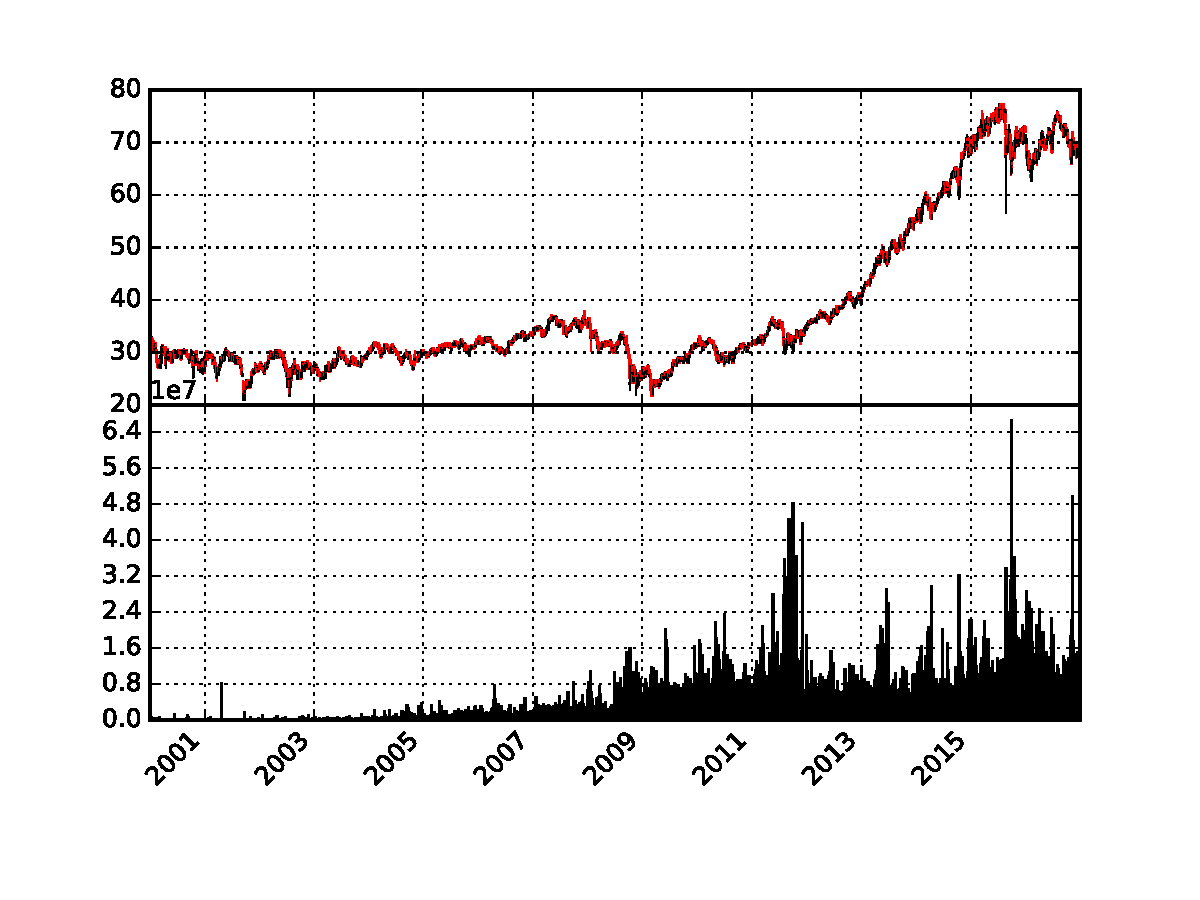
\includegraphics[width=3in]{Images/XLV_raw.pdf}
    % } \\
    % \subfloat[SPY]{
        % 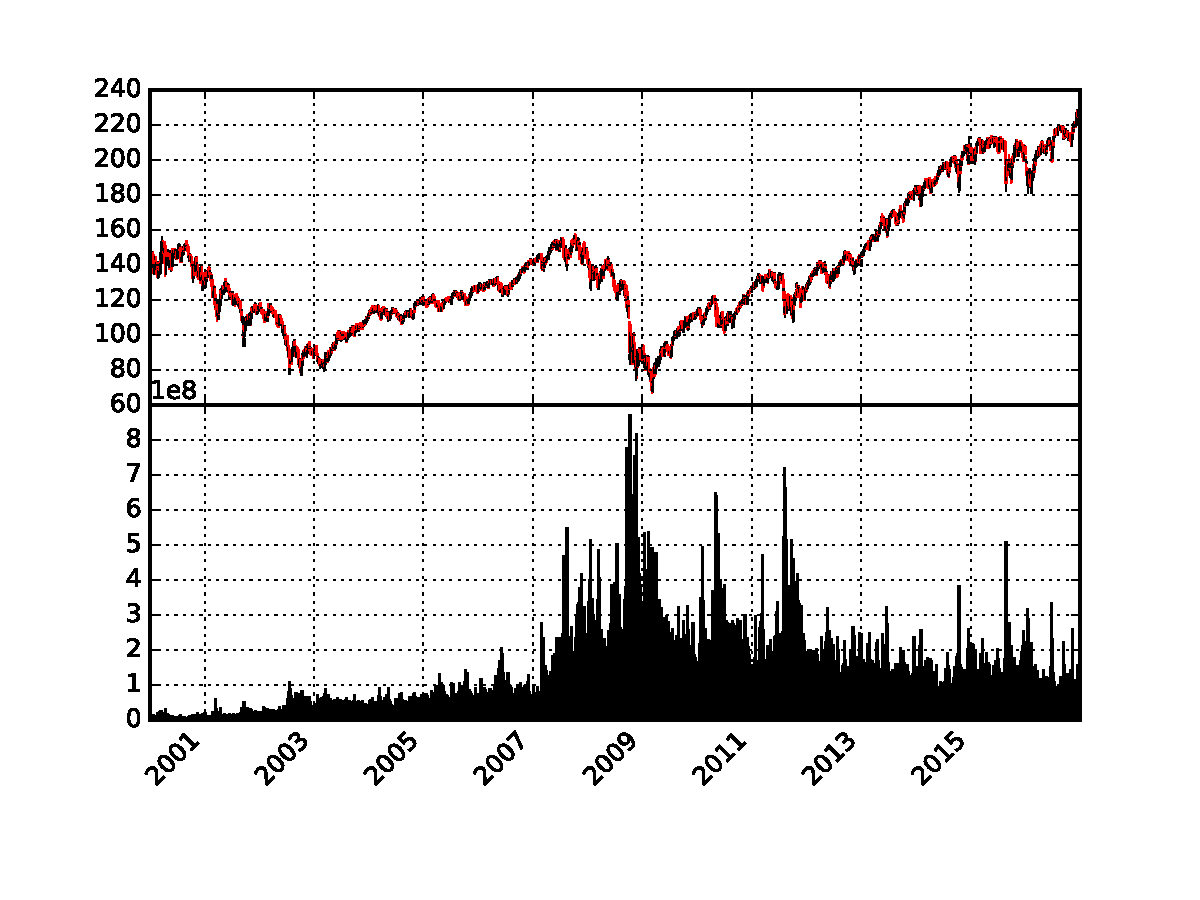
\includegraphics[width=3in]{Images/SPY_raw.pdf}
    % }
    \caption{Raw data visualization}
  \label{plotRawData}
\end{figure}

\subsection{Predictors}
In this project, I explored two different types of methods to predict the
direction of ETF movement: pure data-driven method, and
indicator-driven method.

\textbf{Pure data-driven method.} 1-day lagged version of all the OHLC prices,
volume data and weekday information is used to predict the market direction of
the second day. For example, if we would like to predict the market direction
on 11/30/2010, the predictors are OHLC prices and volume data on 11/29/2010.
Weekday information is treated as dummy variables.

\textbf{Indicator-driven method.} Based on previous studies, it is hypothesized
that various technical indicators can be used as predictors to construct models
to forecast the direction of ETF price. After reviewing prior
publications\cite{Fundreport, thesis, plosone, arXiv, trade}, 16 technical
indicators are chosen as predictor in constructing prediction models in this
project. Table 1 lists selected technical indicators and parameters used. For
some technical indicators, i.e. EWMV and Disparity Index, multiple parameters
(days) are used to calculate these technical indicators. Therefore, there are
19 input techinical indicators in total.Weekday information is also included in
this method.

 \begin{table}
   \centering
   \caption{Selected technical indicators and their parameters}
   \label{technicalIndicators}
    \begin{tabular}{ll}
      \hline
      Technical indicators                         & Parameters     \\
      \hline
      Exponential Weighted Moving Average (EWMA)   & 7, 50, 200 days \\
      Moving Average Convergence/Divergence (MACD) & 12\&26 days     \\
      Relative Strength Index (RSI)                & 14 days         \\
      Average Directional Index (ADX)              & 14 days         \\
      Fast Stochastic Oscillator \%K               & 14 days         \\
      Fast Stochastic Oscillator \%D               & 14 days         \\
      Slow Stochastic Oscillator \%K               & 3 days          \\
      Momentum                                     & 4 days          \\
      Acceleration                                 & 5\&34\&5 days   \\
      William's R                                  & 14 days         \\
      Accumulation/Distribution                    & NA              \\
      Chaikin Oscillator                           & 3\&10 days      \\
      William Accumulation/Distribution            & NA              \\
      On Balance Volume                            & NA              \\
      Disparity Index                              & 5, 10 days      \\
      Commodity Channel Index (CCI)                & 14 days         \\
      \hline
    \end{tabular}
\end{table}

\subsection{Prediction Models}
The purpose of the project is to predict the direction of ETF movement. The
direction is determined by Close and Open prices of the same day.
The relationship between Close and Open prices is transformed to three
different types in order to be predicted in different models:

\begin{itemize}
  \item \textbf{Type I: binary.} If the close price is higher that the open
    price of the same day, the direction is labeled “1”. Otherwise labeled “0”.
    In order to predict binary data, classification models need to be
    implemented.
  \item \textbf{Type II: Percentage.} The equation to calculate the percentage
    is $Percentage = \frac {P_{close} - P_{Open}} {P_{Open}}$. It can be
    predicted using regression models. Then the percentage can be converted to
    directions: if Percentage is positive, it means the price is going up.
    Otherwise, it is going down.
  \item \textbf{Type III: Ratio.} The equation to calculate the ratio is
    $Ratio = \frac {P_{close}} {P_{Open}}$. It can be predicted using
    regression models as well. Then the ratio can be converted back to
    directions: if Ratio > 1, it means the price is going up.
    Otherwise, it is going down.
\end{itemize}

The following four types of models are implemented in the project based on
different data types of the dependent variable.

\textbf{Logistic Regression.} The logistic regression model can be used to
predict the direction directly. I consider both L1 and L2 penalties in the
model. The difference between L1 and L2 penalty is that L1 penalty can yield a
sparse coefficient vector while L2 penalty cannot. However, the limitation for
the L1 penalty is that if the predictors have high correlation, the L1 penalty
can only select one of them. This can make the model miss useful information
and thus has a negative effect on the prediction accuracy.

Hyerparameter search space in this model:
\begin{itemize}
  \item $C$(L1 regularization term): \{2, 5, 10, 20, 30, 40, 50, 60, 70, 80,
    90, 100\}
  \item $C$(L2 regularization term): \{2, 5, 10, 20, 30, 40, 50, 60, 70, 80,
    90, 100\}
\end{itemize}

\textbf{Lasso Regression.} Lasso regression model is a regression model using
L1 regularization. It is applied to predict the ratio/percentage.

Hyerparameter search space in this model:
\begin{itemize}
  \item $\alpha$(L1 regularization term): \{0.1, 1, 5, 10, 30, 50, 100\}
\end{itemize}

\textbf{Ridge Regression.} Ridge regression is a regression model using L2
regularization. It is also applied to predict the ratio/percentage.

Hyerparameter search space in this model:
\begin{itemize}
  \item $\alpha$(L1 regularization term): \{0.1, 1, 5, 10, 30, 50, 100\}
\end{itemize}

\textbf{Artificial Neural Network.} The artificial neural network implemented
here is a multiple perceptron (MLP). It maps sets of input data onto a set of
outputs. The MLP model in this project contains an input layer, a hidden layer,
and an output layer, each of which is connected to the other in the same
sequence as listed above. The input layer corresponds to the input predictors.
The hidden layers is used for capturing the nonlinear relationships among
predictors. The output layer consists of only one neuron that represents the
predicted direction/ratio/percentage.

Hyerparameter search space in the MLP model:
\begin{itemize}
  \item $\alpha$(L2 regularization term): \{0.1, 1, 5, 10, 30, 50, 100\}
  \item Hidden layers: \{(9), (6), (3)\}
\end{itemize}

Figure \ref{combinations} summarizes the combinations of input predictors, the dependent
variable and models. In total, there are 18 combinations.

\begin{figure}
  \centering
    \subfloat[Data-driven method]{
        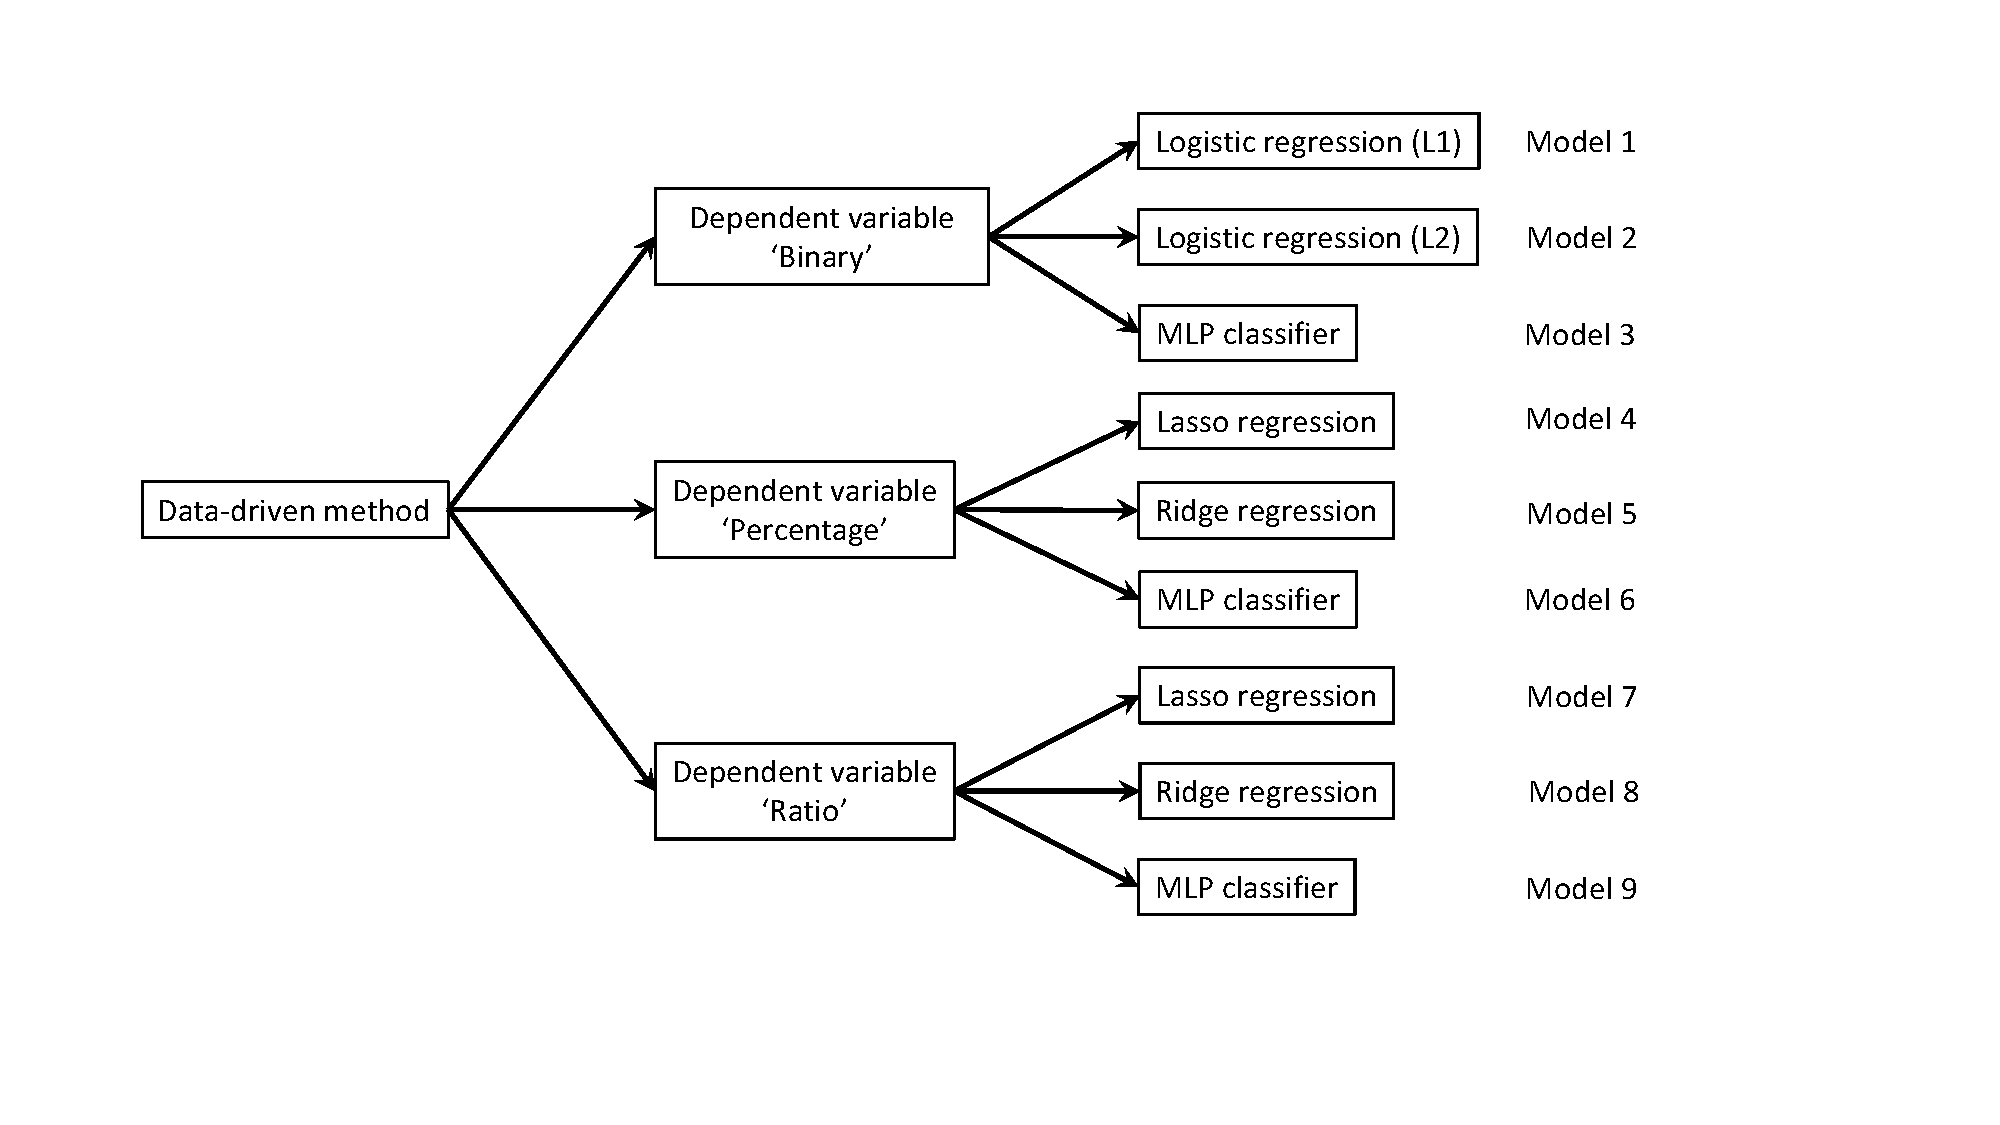
\includegraphics[width=5in]{Images/combinations1.pdf}
    } \\
    \subfloat[Indication-driven method]{
        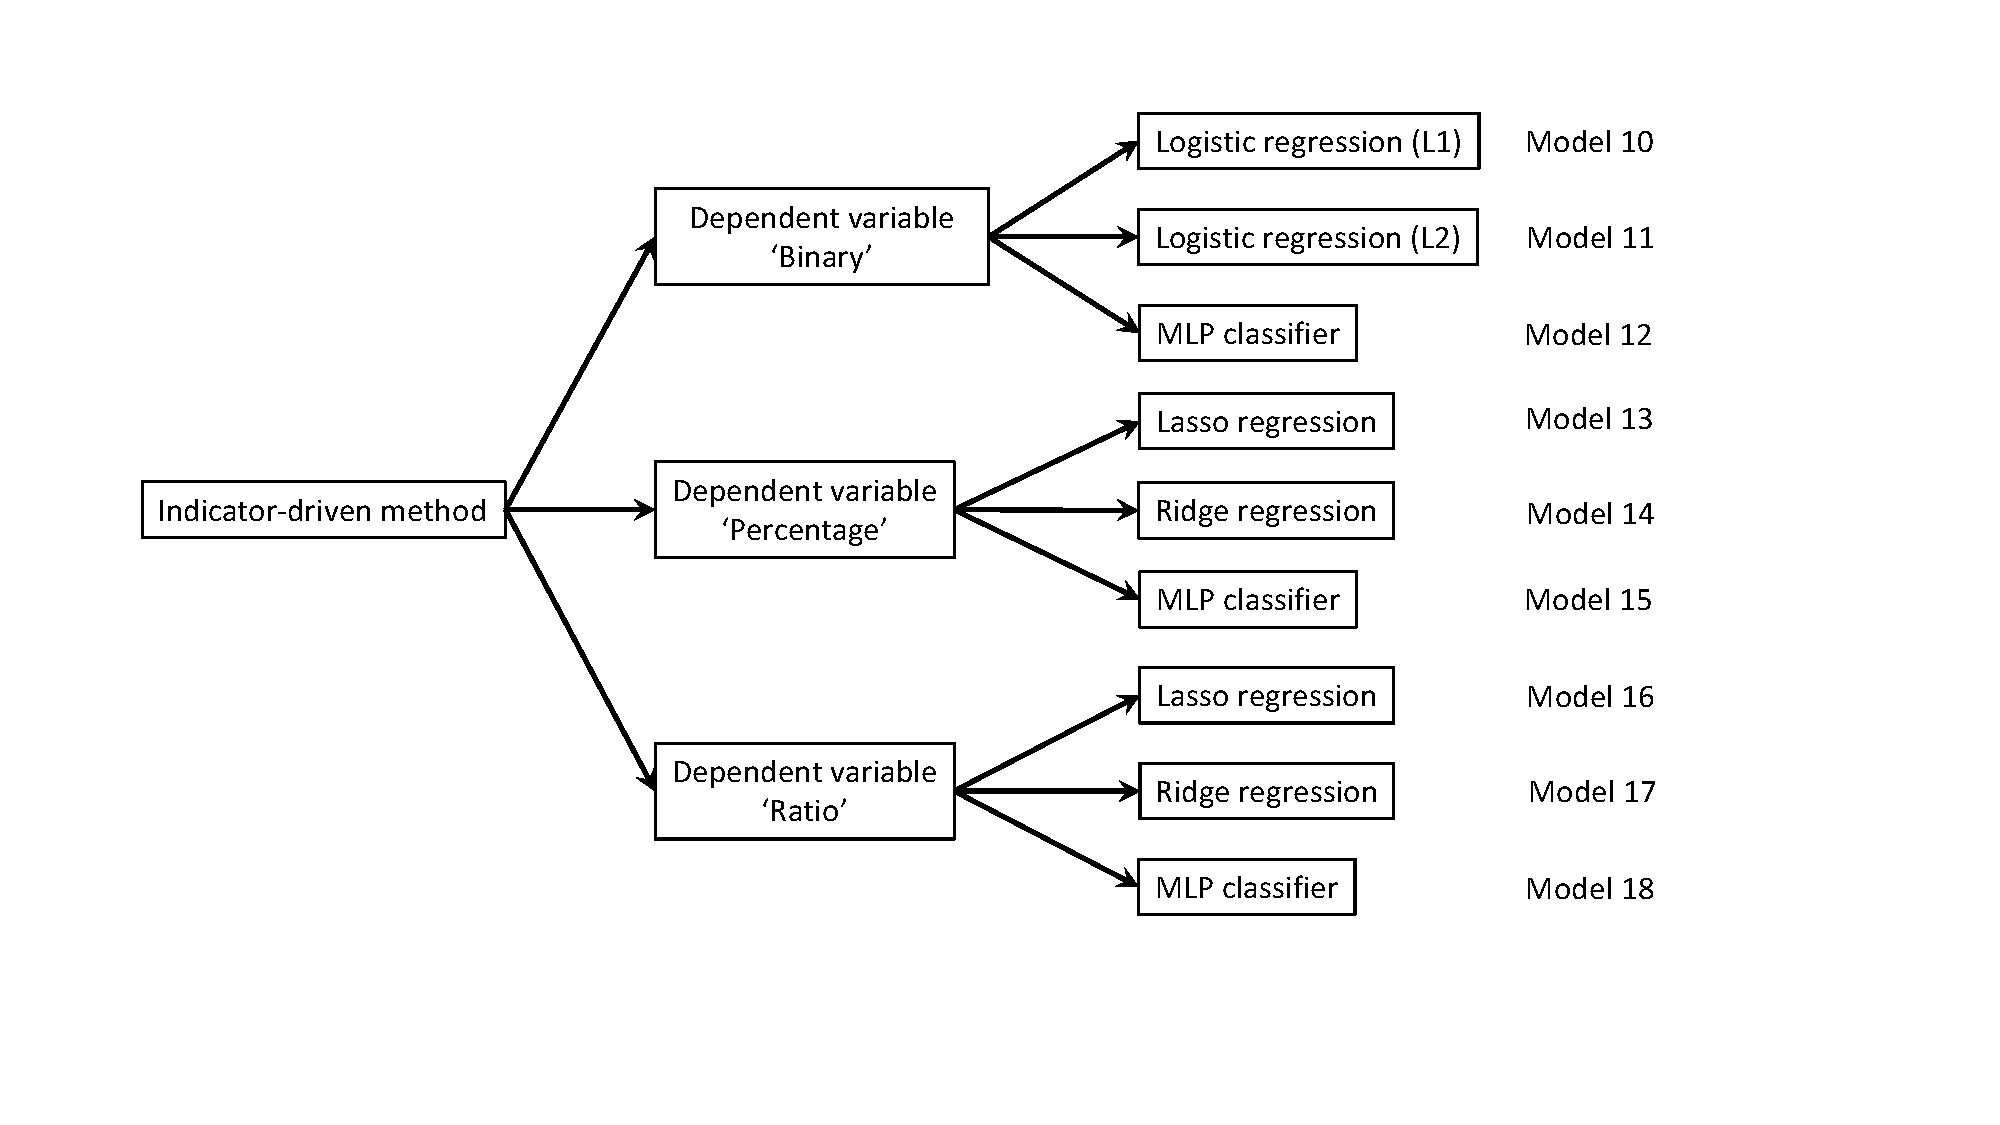
\includegraphics[width=5in]{Images/combinations2.pdf}
    } \\
  \caption{The combinations of input predictors, the dependent variable and
  models}
  \label{combinations}
\end{figure}

\subsection{Performance Measurement}
In the project, I am only interested in forecasting the direction of the
ETF movement. Therefore, after doing prediction using the percentage/ratio
dependent variable, I transform the predicted results to binary results as
well. That is, if the predicted percentage is positive, the direction label is
“1”; otherwise, it is “0”. If the predicted ratio is large than 1, the
direction label is “1”; otherwise, it is “0”.

The prediction performance is evaluated by using the following equations:

\begin{equation}
  P_t =
  \begin{cases}
    1, y_t - \hat{y_t} = 0\\
    0, y_t - \hat{y_t} \neq 0
  \end{cases}
\end{equation}

where $y_t$ is the actual direction of the ETF movement for the ith
trading day, while $\hat{y_t}$ donates the predicted direction for the ith
trading day.

$$Accuracy = \frac {1} {N} \sum_{t=1}^{N} P_t, t = 1, 2, 3, \dots, n$$

where $N$ is the total number of predicted results.

\subsection{Prediction Process}
After retrieving ETF data from Yahoo Finance and calculating input predictors.
I plug in the data into the above 18 models to forecast the future direction of
ETF, and compare the performance of each model. I conduct the prediction
process as follows:

\begin{enumerate}
  \item Calculate all indicators using all data from January 1st 2000 to
    December 31st 2016. And discard all samples including NaN.
  \item Divide data into training data and test data as described in Data
    section.
  \item Normalize data by removing the mean value of each predictor, and scale
    it by dividing by its standard deviation. In order to avoid incorporating
    information from test data into training process, I only use the mean value
    and standard deviation of training data to normlize all data.
  \item Use training data to train models. In order to tune hyerparameters in
    models and avoid over-fitting, 10-fold crossing validation is implemented
    in training process. Since the data is time series and indicator
    calculation depends on prices and volume size of passing days, I use
    forward chaining procedure to avoid incorporating test data into training
    process. The forward chaining procedure is like:
    \begin{enumerate}
      \item fold 1: training [1], test [2]
      \item fold 2: training [1 2], test [3] \\
        \dots
      \item fold 9: training [1 2 3 \dots 9], test [10]
    \end{enumerate}
  \item Predict the next day's ETF movement using each model with the best
    hyerparameters, and compare their performance.
\end{enumerate}

\section{Experimental Results}

\subsection{Prediction Accuracy}
To evaluate the performance of each model, I used out-of-sample data which
ranges from January 1st 2016 to December 31st 2016. Figure \ref{accuracy}
shows the performance of each model on each ETF sector. The model with best
accuracy for each dataset is marked with a square.

It shows that the best prediction accuracy of each ETF sector ranges from
0.55 to 0.6, which means at least one predictive model can gain some
information in forecasting the direction of ETF movement. For some ETF sectors,
such as XLE, XLU, XLK, XLY, XLV, the pure data-driven method can achieve a
better result, while the indicator-driven method is superior in predicting some
other ETF sectors' movement, including XLB, XLP, and SPY. In addition, the
performance has no difference in forecasting XLI movement by either data-driven
or indicator-driven method. Moreover, predicting either “Binary” or
“Percentage”/“Ratio” can achieve good accuracy depending on the dataset. The
prediction accuracy has no preference for MLP or regression models.

\begin{figure}
  % \centering
    \subfloat[XLE]{
        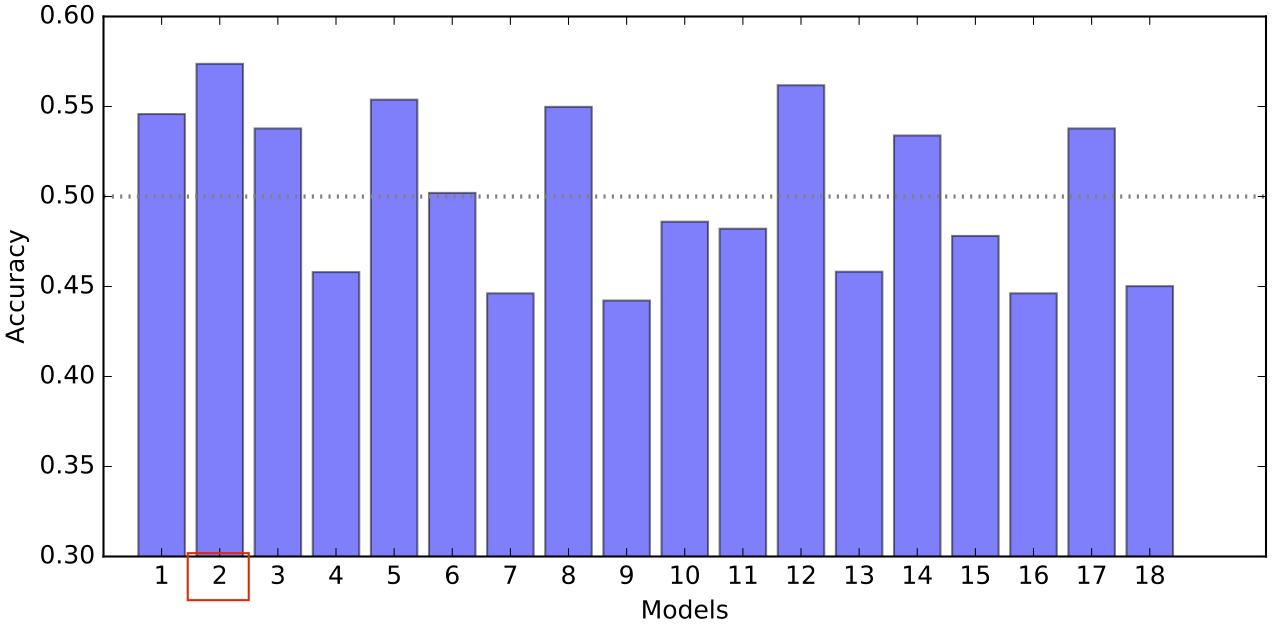
\includegraphics[width=3in]{Images/XLE_accuracy.png}
    }
    \subfloat[XLU]{
        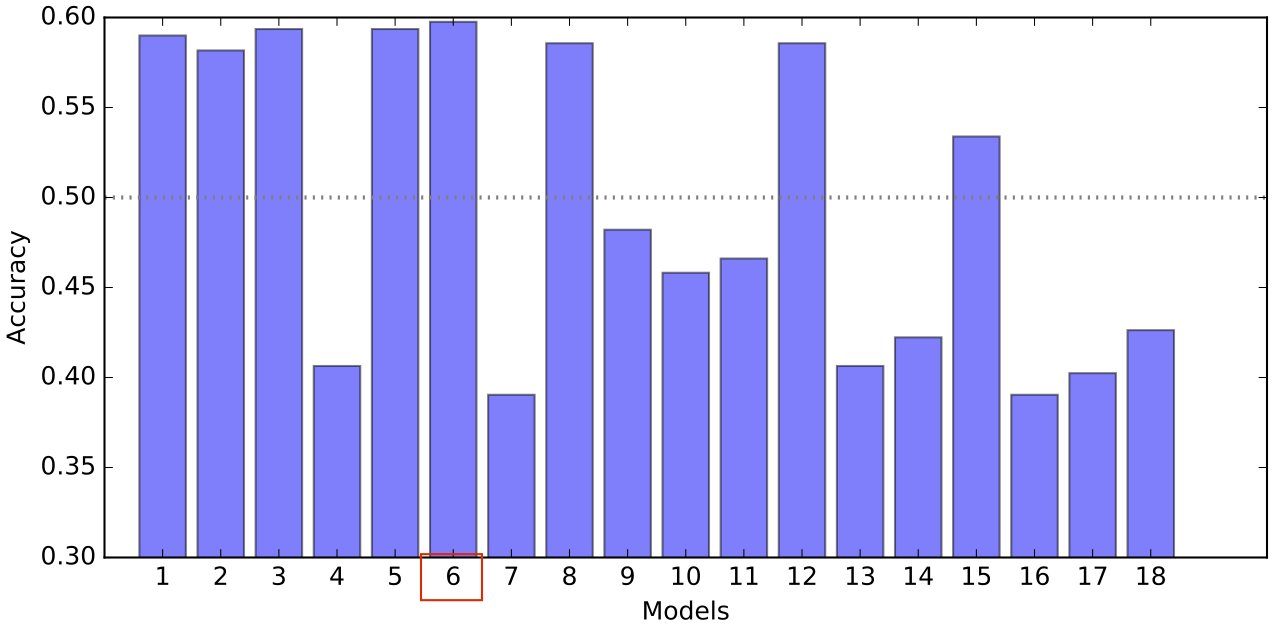
\includegraphics[width=3in]{Images/XLU_accuracy.png}
    } \\
    \subfloat[XLK]{
        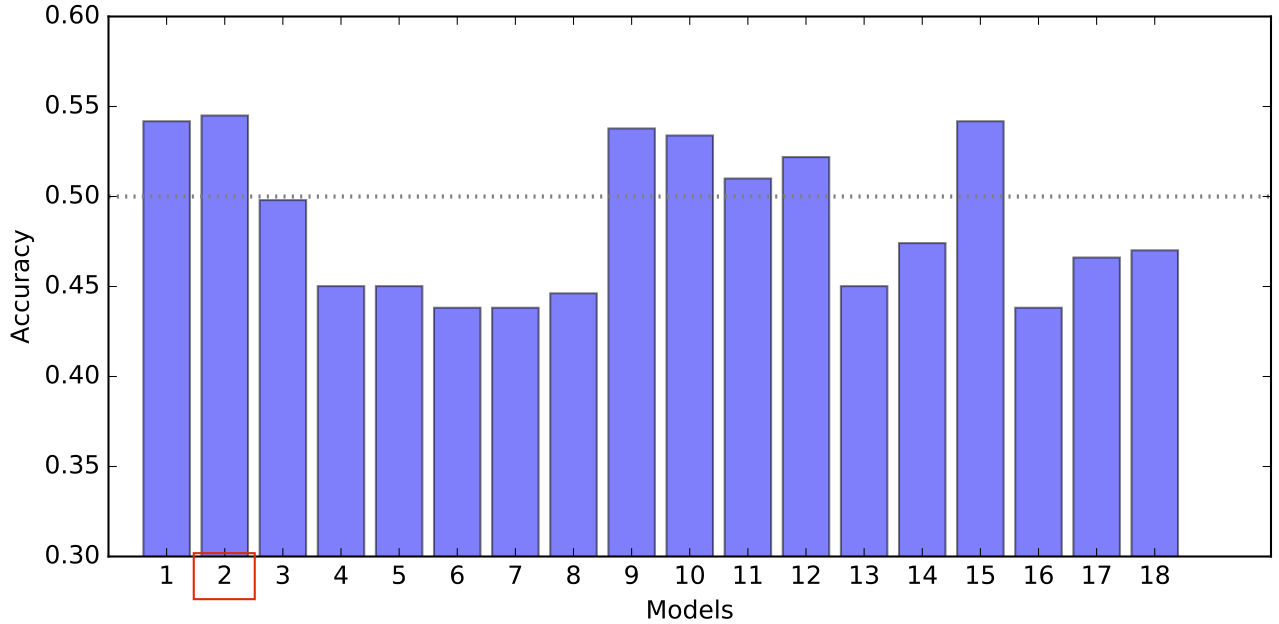
\includegraphics[width=3in]{Images/XLK_accuracy.png}
    }
    \subfloat[XLB]{
        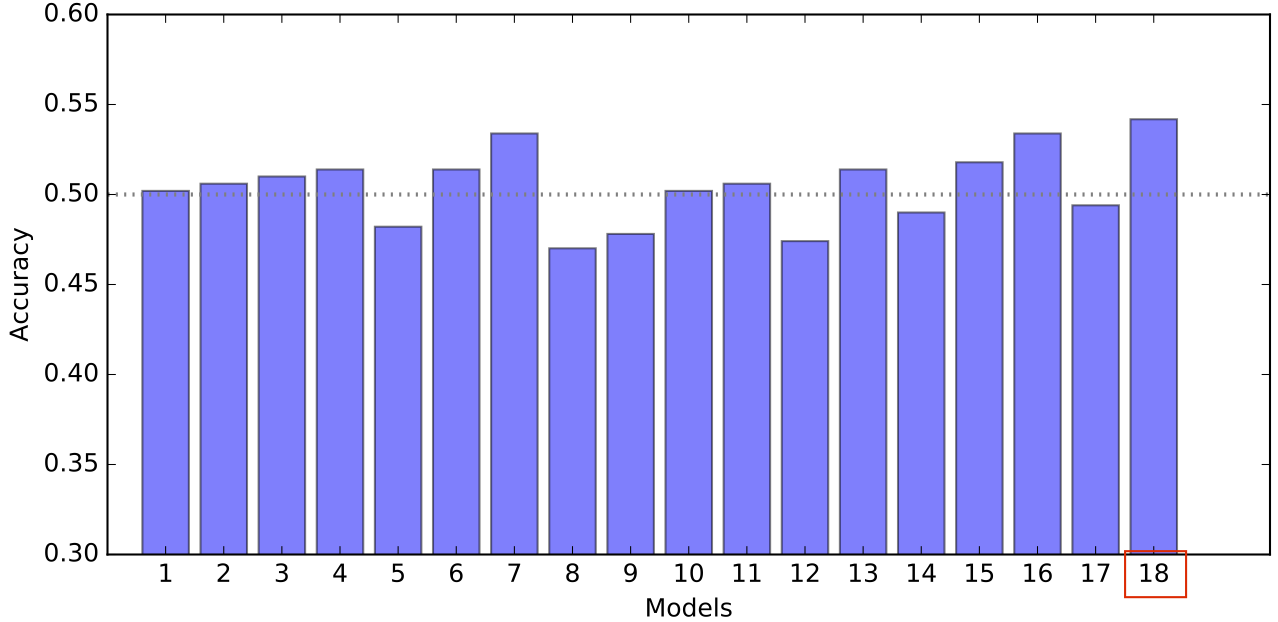
\includegraphics[width=3in]{Images/XLB_accuracy.png}
    } \\
    \subfloat[XLP]{
        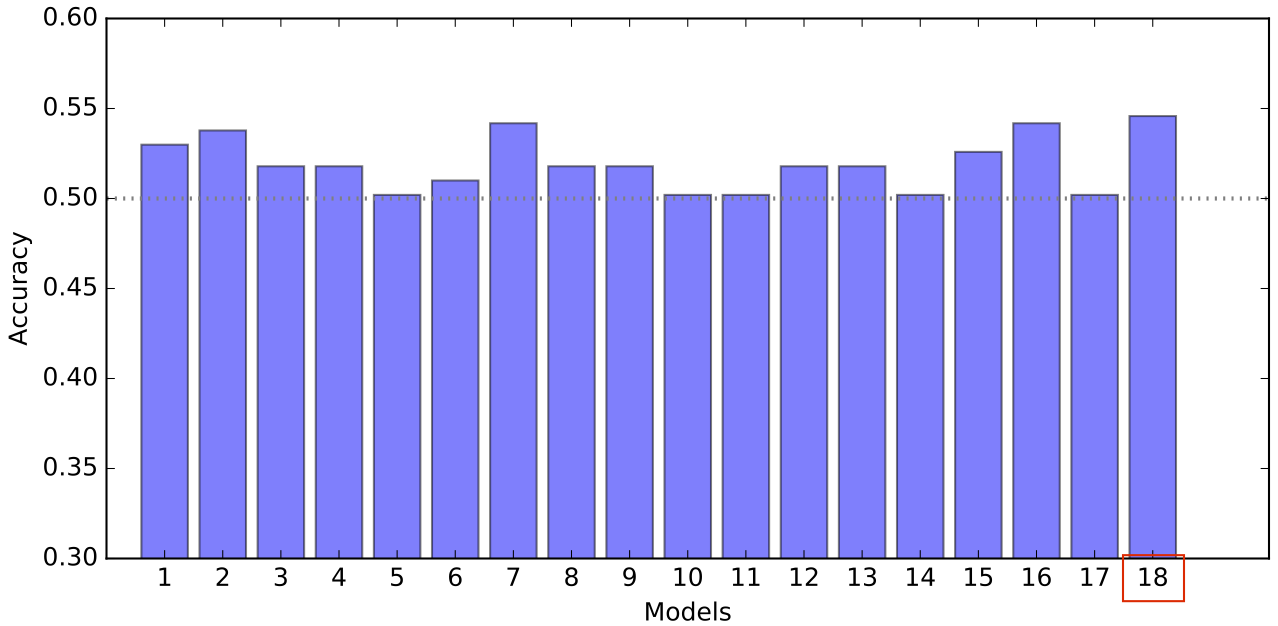
\includegraphics[width=3in]{Images/XLP_accuracy.png}
    }
    \subfloat[XLY]{
        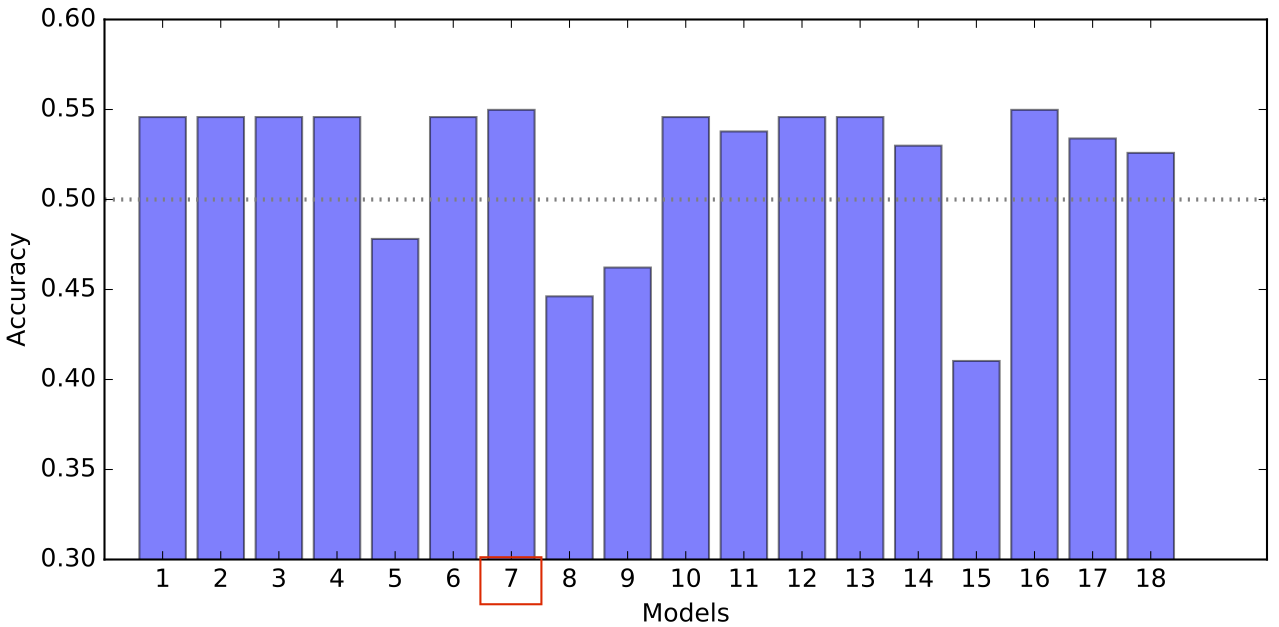
\includegraphics[width=3in]{Images/XLY_accuracy.png}
    } \\
  % \caption{The performance of each model on ETF forecasting}
  % % \label{accuracy}
% \end{figure}
% \begin{figure}
  % \ContinuedFloat
  % \centering
    \subfloat[XLI]{
        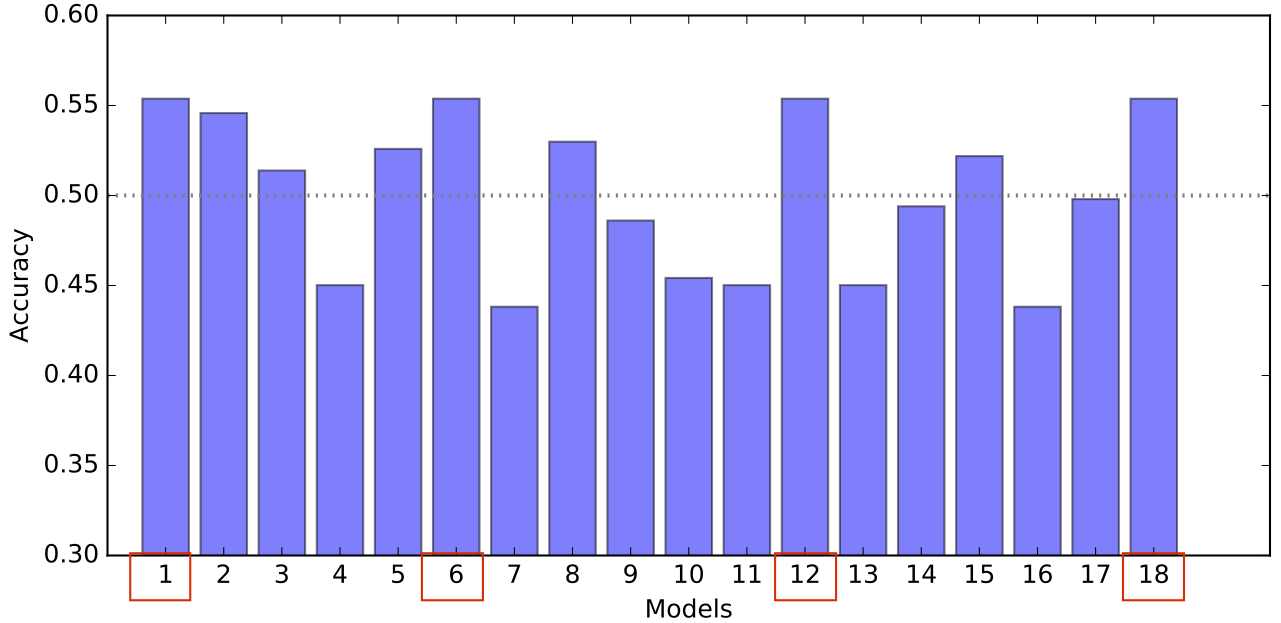
\includegraphics[width=3in]{Images/XLI_accuracy.png}
    }
    \subfloat[XLV]{
        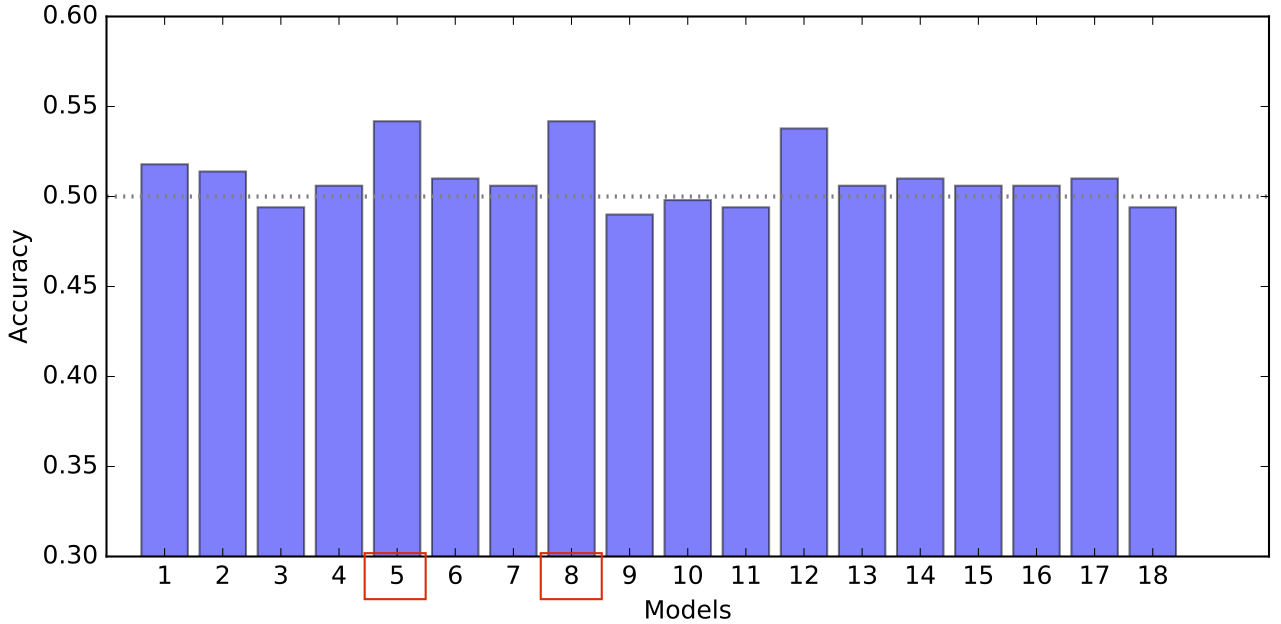
\includegraphics[width=3in]{Images/XLV_accuracy.png}
    } \\
    \subfloat[SPY]{
        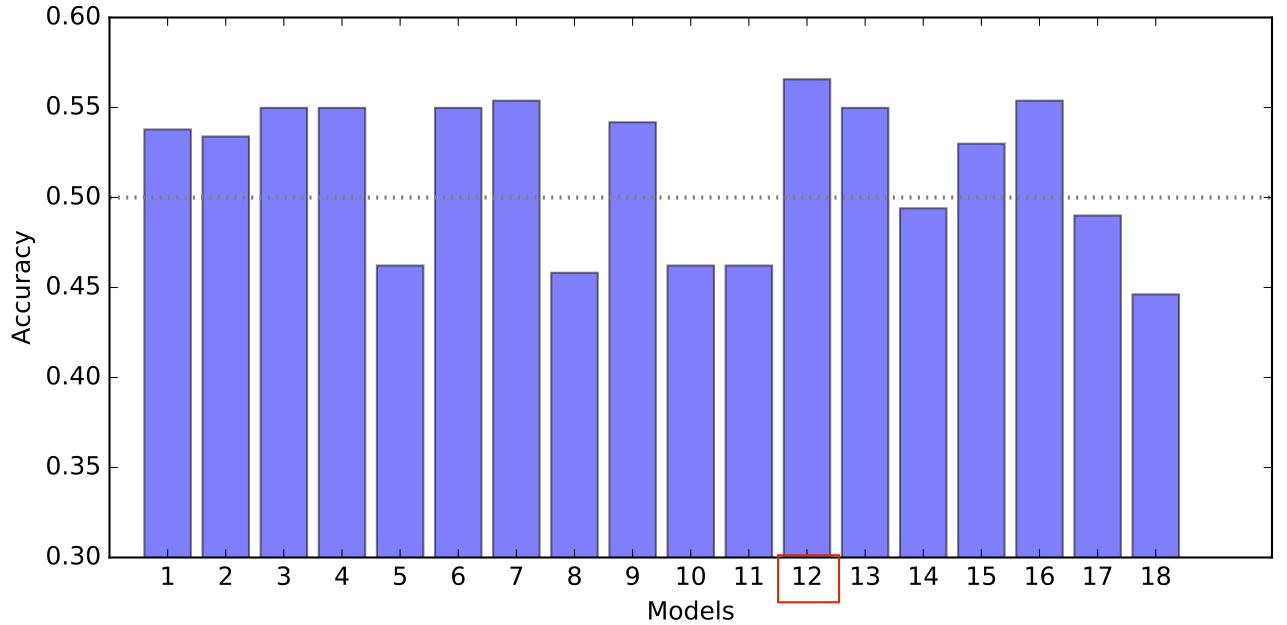
\includegraphics[width=3in]{Images/SPY_accuracy.png}
    }
    \caption{The performance of each model on ETF forecasting (Continue)}
  \label{accuracy}
\end{figure}
\clearpage
 % \begin{table}
   % \centering
   % \caption{The performance of each model on ETF prediction}
   % \label{performance}
   % \subfloat[XLE] {
      % \begin{tabular}{lll}
        % \hline
        % Models    & Accuracy               & Hyerparameters\\
        % \hline
        % Model 1   & 54.58\%                & 5             \\
        % Model 2   & \textbf{57.37\%}       & 5             \\
        % Model 3   & 53.78\%                & (6), 1        \\
        % Model 4   & 45.80\%                & 100           \\
        % Model 5   & 55.38\%                & 0.1           \\
        % Model 6   & 50.20\%                & (6), 1        \\
        % Model 7   & 44.62\%                & 100           \\
        % Model 8   & 54.98\%                & 0.1           \\
        % Model 9   & 44.22\%                & (9), 0.1      \\
        % Model 10  & 48.60\%                & 10            \\
        % Model 11  & 48.21\%                & 40            \\
        % Model 12  & 56.18\%                & (3), 5        \\
        % Model 13  & 45.82\%                & 100           \\
        % Model 14  & 53.39\%                & 1             \\
        % Model 15  & 47.81\%                & (9), 0.1      \\
        % Model 16  & 44.62\%                & 100           \\
        % Model 17  & 53.78\%                & 1             \\
        % Model 18  & 45.02\%                & (9), 0.1      \\
        % \hline
      % \end{tabular}
    % }
   % \subfloat[XLU] {
      % \begin{tabular}{lll}
        % \hline
        % Models    & Accuracy               & Hyerparameters\\
        % \hline
        % Model 1   & 59.00\%                & 2             \\
        % Model 2   & 58.17\%                & 2             \\
        % Model 3   & 59.36\%                & (3), 5        \\
        % Model 4   & 40.64\%                & 100           \\
        % Model 5   & 59.36\%                & 0.1           \\
        % Model 6   & \textbf{59.76}\%       & (3), 5        \\
        % Model 7   & 39.04\%                & 100           \\
        % Model 8   & 58.57\%                & 0.1           \\
        % Model 9   & 48.21\%                & (6), 1        \\
        % Model 10  & 45.82\%                & 2             \\
        % Model 11  & 46.61\%                & 2             \\
        % Model 12  & 58.57\%                & (3), 5        \\
        % Model 13  & 40.64\%                & 100           \\
        % Model 14  & 42.23\%                & 10            \\
        % Model 15  & 53.39\%                & (6), 1        \\
        % Model 16  & 39.04\%                & 100           \\
        % Model 17  & 40.24\%                & 5             \\
        % Model 18  & 42.63\%                & (6), 1        \\
        % \hline
      % \end{tabular}
    % } \\
   % \subfloat[XLK] {
      % \begin{tabular}{lll}
        % \hline
        % Models    & Accuracy               & Hyerparameters\\
        % \hline
        % Model 1   & 54.18\%                & 5             \\
        % Model 2   & 54.50\%                & 2             \\
        % Model 3   & 49.80\%                & (6), 1        \\
        % Model 4   & 45.02\%                & 100           \\
        % Model 5   & 45.02\%                & 10            \\
        % Model 6   & 43.82\%                & (9), 0.1      \\
        % Model 7   & 43.82\%                & 100           \\
        % Model 8   & 44.62\%                & 10            \\
        % Model 9   & 53.78\%                & (9), 0.1      \\
        % Model 10  & 53.39\%                & 2             \\
        % Model 11  & 51.00\%                & 20            \\
        % Model 12  & 52.19\%                & (9), 0.1      \\
        % Model 13  & 45.02\%                & 100           \\
        % Model 14  & 47.41\%                & 100           \\
        % Model 15  & 54.18\%                & (3), 5        \\
        % Model 16  & 43.82\%                & 100           \\
        % Model 17  & 46.61\%                & 10            \\
        % Model 18  & 47.01\%                & (6), 1        \\
        % \hline
      % \end{tabular}
    % }
   % \subfloat[XLB] {
      % \begin{tabular}{lll}
        % \hline
        % Models    & Accuracy               & Hyerparameters\\
        % \hline
        % Model 1   & 50.20\%                & 100           \\
        % Model 2   & 50.60\%                & 5             \\
        % Model 3   & 51.00\%                & (3), 5        \\
        % Model 4   & 51.39\%                & 100           \\
        % Model 5   & 48.21\%                & 0.1           \\
        % Model 6   & 51.39\%                & (3), 5        \\
        % Model 7   & 53.39\%                & 100           \\
        % Model 8   & 47.01\%                & 0.1           \\
        % Model 9   & 47.81\%                & (3), 5        \\
        % Model 10  & 50.20\%                & 90            \\
        % Model 11  & 50.60\%                & 100           \\
        % Model 12  & 47.41\%                & (6), 1        \\
        % Model 13  & 51.39\%                & 100           \\
        % Model 14  & 49.00\%                & 1             \\
        % Model 15  & 51.79\%                & (3), 5        \\
        % Model 16  & 53.39\%                & 100           \\
        % Model 17  & 49.40\%                & 1             \\
        % Model 18  & 54.18\%                & (6), 1        \\
        % \hline
      % \end{tabular}
    % } \\
% \end{table}
 % \begin{table}
   % \centering
   % \ContinuedFloat
   % \caption{The performance of each model on ETF prediction (continue)}
   % \label{performance}
   % \subfloat[XLP] {
      % \begin{tabular}{lll}
        % \hline
        % Models    & Accuracy               & Hyerparameters\\
        % \hline
        % Model 1   & 52.99\%                & 20            \\
        % Model 2   & 53.78\%                & 5             \\
        % Model 3   & 51.79\%                & (6), 1        \\
        % Model 4   & 51.79\%                & 100           \\
        % Model 5   & 50.20\%                & 1             \\
        % Model 6   & 51.00\%                & (3), 5        \\
        % Model 7   & 54.18\%                & 100           \\
        % Model 8   & 51.79\%                & 1             \\
        % Model 9   & 51.79\%                & (9), 0.1      \\
        % Model 10  & 50.20\%                & 70            \\
        % Model 11  & 50.20\%                & 80            \\
        % Model 12  & 51.79\%                & (9), 0.1      \\
        % Model 13  & 51.79\%                & 100           \\
        % Model 14  & 50.20\%                & 100           \\
        % Model 15  & 52.59\%                & (9), 0.1      \\
        % Model 16  & 54.18\%                & 100           \\
        % Model 17  & 50.20\%                & 100           \\
        % Model 18  & 54.58\%                & (9), 0.1      \\
        % \hline
      % \end{tabular}
    % }
   % \subfloat[XLY] {
      % \begin{tabular}{lll}
        % \hline
        % Models    & Accuracy               & Hyerparameters\\
        % \hline
        % Model 1   & 54.58\%                & 10            \\
        % Model 2   & 54.58\%                & 2             \\
        % Model 3   & 54.58\%                & (6), 1        \\
        % Model 4   & 54.58\%                & 100           \\
        % Model 5   & 47.81\%                & 50            \\
        % Model 6   & 54.58\%                & (3), 5        \\
        % Model 7   & 54.98\%                & 100           \\
        % Model 8   & 44.62\%                & 0.1           \\
        % Model 9   & 46.22\%                & (6), 1        \\
        % Model 10  & 54.58\%                & 100           \\
        % Model 11  & 53.78\%                & 70            \\
        % Model 12  & 54.58\%                & (3), 3        \\
        % Model 13  & 54.58\%                & 100           \\
        % Model 14  & 52.99\%                & 1             \\
        % Model 15  & 41.03\%                & (9), 0.1      \\
        % Model 16  & 54.98\%                & 100           \\
        % Model 17  & 53.39\%                & 1             \\
        % Model 18  & 52.59\%                & (9), 0.1      \\
        % \hline
      % \end{tabular}
    % } \\
   % \subfloat[XLI] {
      % \begin{tabular}{lll}
        % \hline
        % Models    & Accuracy               & Hyerparameters\\
        % \hline
        % Model 1   & 55.38\%                & 100          \\
        % Model 2   & 54.58\%                & 5            \\
        % Model 3   & 51.39\%                & (9), 0.1     \\
        % Model 4   & 45.02\%                & 100          \\
        % Model 5   & 52.59\%                & 1            \\
        % Model 6   & 55.38\%                & (6), 1       \\
        % Model 7   & 43.82\%                & 100          \\
        % Model 8   & 52.99\%                & 1            \\
        % Model 9   & 48.61\%                & (6), 1       \\
        % Model 10  & 45.42\%                & 2            \\
        % Model 11  & 45.02\%                & 2            \\
        % Model 12  & 55.38\%                & (6), 1       \\
        % Model 13  & 45.02\%                & 100          \\
        % Model 14  & 49.40\%                & 100          \\
        % Model 15  & 52.19\%                & (9), 0.1     \\
        % Model 16  & 43.82\%                & 100          \\
        % Model 17  & 49.80\%                & 100          \\
        % Model 18  & 55.38\%                & (6), 1       \\
        % \hline
      % \end{tabular}
    % }
   % \subfloat[XLV] {
      % \begin{tabular}{lll}
        % \hline
        % Models    & Accuracy               & Hyerparameters\\
        % \hline
        % Model 1   & 51.79\%                & 90            \\
        % Model 2   & 51.39\%                & 60            \\
        % Model 3   & 49.40\%                & (3), 5        \\
        % Model 4   & 50.60\%                & 100           \\
        % Model 5   & 54.18\%                & 0.1           \\
        % Model 6   & 51.00\%                & (9), 0.1      \\
        % Model 7   & 50.60\%                & 100           \\
        % Model 8   & 54.18\%                & 0.1           \\
        % Model 9   & 49.00\%                & (6), 1        \\
        % Model 10  & 49.80\%                & 5             \\
        % Model 11  & 49.40\%                & 60            \\
        % Model 12  & 53.78\%                & (6), 1       \\
        % Model 13  & 50.60\%                & 100          \\
        % Model 14  & 51.00\%                & 100          \\
        % Model 15  & 50.60\%                & (3), 5      \\
        % Model 16  & 50.60\%                & 100          \\
        % Model 17  & 51.00\%                & 100          \\
        % Model 18  & 49.40\%                & (9), 0.1       \\
        % \hline
      % \end{tabular}
    % } \\
% \end{table}
 % \begin{table}
   % \centering
   % \ContinuedFloat
   % \caption{The performance of each model on ETF prediction (continue)}
   % \label{performance}
   % \subfloat[SPY] {
      % \begin{tabular}{lll}
        % \hline
        % Models    & Accuracy               & Hyerparameters\\
        % \hline
        % Model 1   & 53.78\%                & 2            \\
        % Model 2   & 53.39\%                & 5            \\
        % Model 3   & 54.98\%                & (3), 5        \\
        % Model 4   & 54.98\%                & 100           \\
        % Model 5   & 46.22\%                & 30           \\
        % Model 6   & 54.98\%                & (3), 5      \\
        % Model 7   & 55.38\%                & 100           \\
        % Model 8   & 45.82\%                & 30           \\
        % Model 9   & 54.18\%                & (6), 1        \\
        % Model 10  & 46.22\%                & 5             \\
        % Model 11  & 46.22\%                & 5            \\
        % Model 12  & 56.57\%                & (6), 1       \\
        % Model 13  & 54.98\%                & 100          \\
        % Model 14  & 49.40\%                & 0.1          \\
        % Model 15  & 52.99\%                & (6), 1     \\
        % Model 16  & 55.38\%                & 100          \\
        % Model 17  & 49.00\%                & 0.1          \\
        % Model 18  & 44.62\%                & (6), 1       \\
        % \hline
      % \end{tabular}
    % } \\
% \end{table}

\subsection{Strategy Evaluation}
From the previous analysis, I determined the best predicting model for each ETF
dataset. In this section, I use the best models to evaluate different trading
strategies. Table \ref{models} lists models used for each ETF sector data, and
their hyerparameter setting. Figure \ref{equity} shows the cumulative daily
portfolio P\&L of each strategy. Apparently, the strategy based on prediction is
better than SPY long-only strategy, which can earn \$0.971 more at the end of
2016. However, it is worse than all long-only strategy, and can earn \$0.547
less money at the end of 2016. Table \ref{sharpe} shows the annualized Sharpe
ratio for each strategy. The strategy based on my prediction is 3.29, which is
higher than that of other two strategies. Based on previous studies, a ratio of
3 or higher is considered excellent. It indicates that the strategy based on my
prediction takes much less risk to achieve the return, though the return is
a little lower than that of all long-only strategy.

\begin{table}
  \centering
  \caption{The best predicting models and hyerparameter setting}
  \label{models}
  \begin{tabular}{lll}
    \hline
    Dataset     & Model             & Hyerparameters \\
    \hline
    XLE         & Model 2           & 5              \\
    XLU         & Model 6           & (3), 5         \\
    XLK         & Model 2           & 2              \\
    XLB         & Model 18          & (6), 1         \\
    XLP         & Model 18          & (9), 0.1       \\
    XLY         & Model 7           & 100            \\
    XLI         & Model 1           & 100            \\
    XLV         & Model 5           & 0.1            \\
    SPY         & Model 12          & (6), 1         \\
    \hline
  \end{tabular}
\end{table}

\begin{figure}
  \centering
      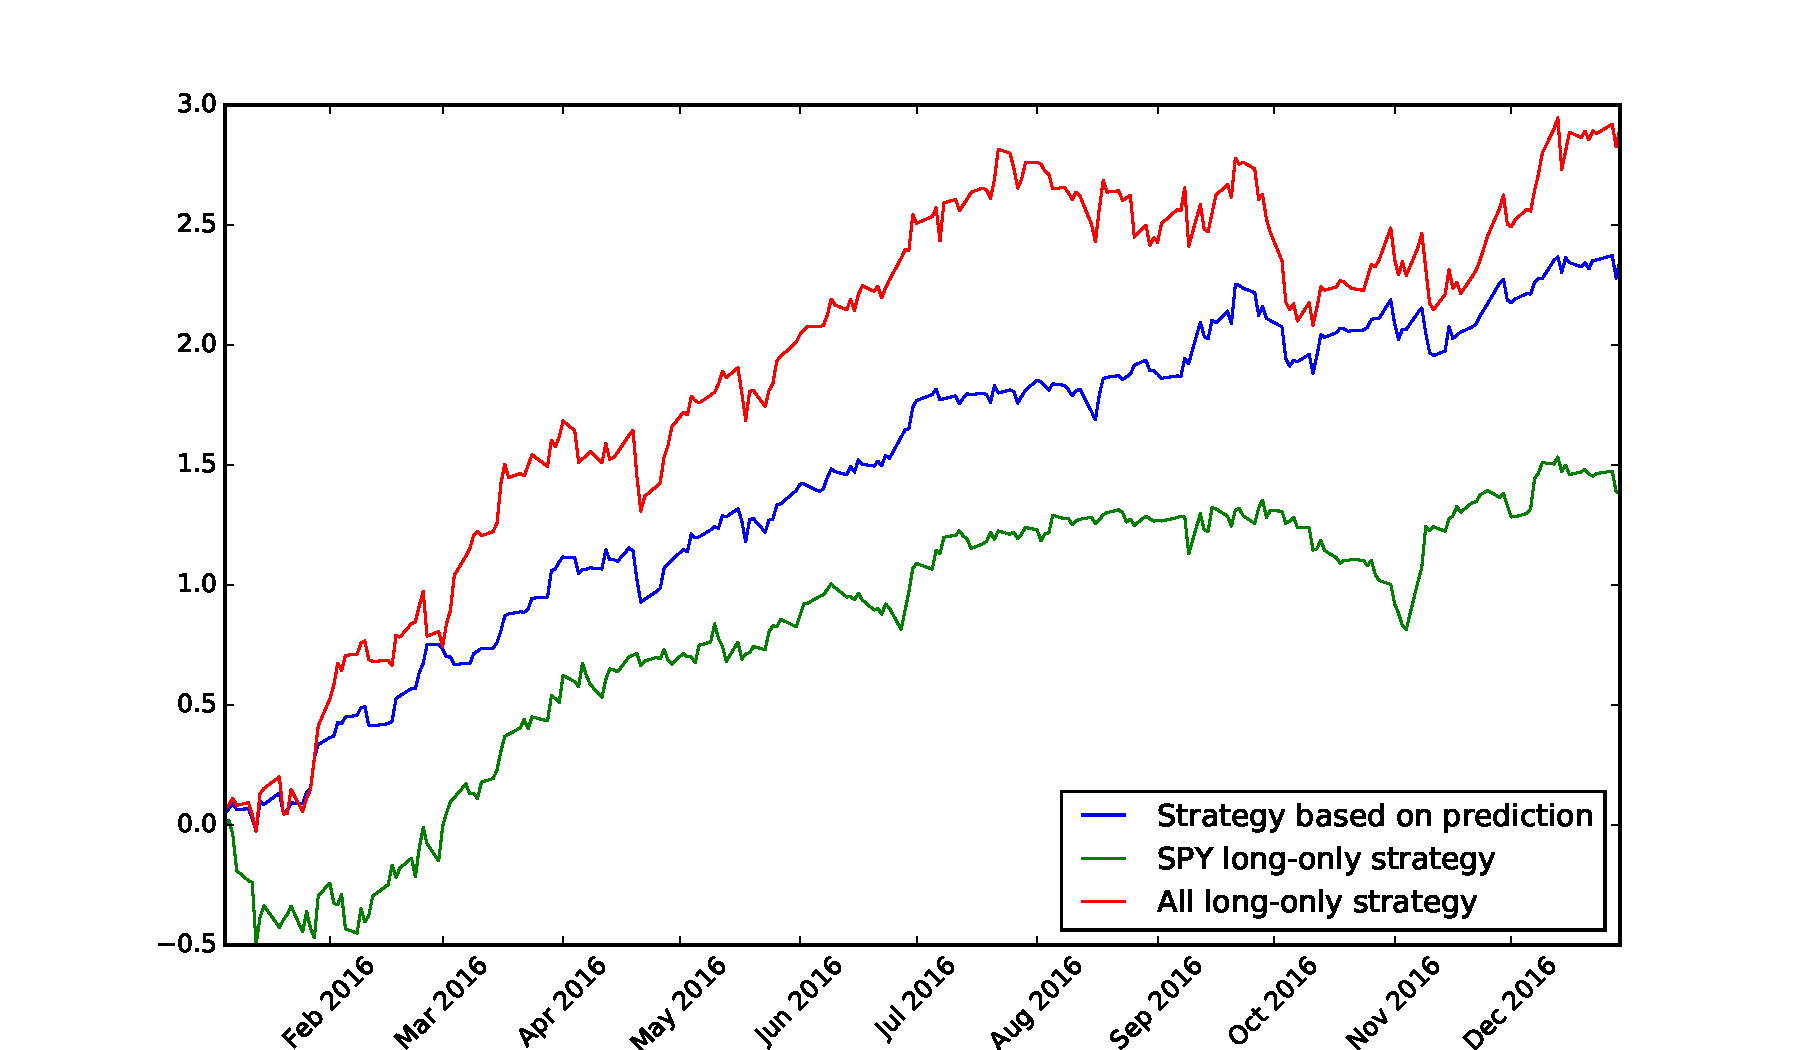
\includegraphics[width=6in]{Images/equity.pdf}
      \caption{Equity curves for each of the three strategies}
      \label{equity}
\end{figure}

% \clearpage

\begin{table}
  \centering
  \caption{The annualized Sharpe ratio for the three strategies}
  \label{sharpe}
  \begin{tabular}{llll}
    \hline
    Strategy & Strategy based on prediction & SPY long-only & All long-only \\
    \hline
    Annualized sharpe ratio & 3.29 & 1.59 & 2.53 \\
    \hline
  \end{tabular}
\end{table}

\section{Conclusion}
In the project, I applied four different models to predict the direction of nine
ETF sectors movement. These models used either different types of dependent
variables or different input predictors. The best predicting accuracy for each
ETF sector ranges from 55\% to 60\%. In addition, the best models for the nine
sectors are different from one another. Therefore, in practice, we should
personalize predictive models for each dataset.

The prediction performance of the models in the project may be improved
further using three methods. The first approach is to use a subset of these
input predictors instead of including all of them in models, especially when
using technical indicators as input predictors. Therefore, optimization
algorithms, such as forward selection, and randomized Lasso/logistic, can be
applied to select predictors with the best prediction power. Besides, other
models, including SVM, ensemble method, can be tested for each dataset. At last, in
the project, I used the percentage of correctly predicted directions to
evaluate the performance of each model. In the future, the trading strategy
(earning) based evaluation can be implemented.
% \clearpage

\section{Source Code}
All project code is available in the following GitHub repository:

\url{https://github.com/KaiUT/ETF_Direction_Prediction}

\bibliographystyle{acm}
\bibliography{reference}
\end{document}
